%%%%%%%%%%%%%%%%%%%%%%%%%%%%%%%%%%%%%%%%%
% a0poster Portrait Poster 
% LaTeX Template
% with University Copenhagen logo
% Version 1.0 (22/06/13)
%
% Based on:
% The a0poster class was created by:
% Gerlinde Kettl and Matthias Weiser (tex@kettl.de)
% 
% This template has been downloaded from:
% http://www.LaTeXTemplates.com
%
%%%%%%%%%%%%%%%%%%%%%%%%%%%%%%%%%%%%%%%%%

%----------------------------------------------------------------------------------------
%	PACKAGES AND OTHER DOCUMENT CONFIGURATIONS
%----------------------------------------------------------------------------------------

\documentclass[a0,portrait]{a0poster}
\usepackage[utf8]{inputenc}

\usepackage{multicol} % This is so we can have multiple columns of text side-by-side
\columnsep=100pt % This is the amount of white space between the columns in the poster
\columnseprule=3pt % This is the thickness of the black line between the columns in the poster

\usepackage[svgnames]{xcolor} % Specify colors by their 'svgnames', for a full list of all colors available see here: http://www.latextemplates.com/svgnames-colors

\usepackage{times} % Use the times font
%\usepackage{palatino} % Uncomment to use the Palatino font
\usepackage{array}
\usepackage{graphicx} % Required for including images
\graphicspath{{figures/}} % Location of the graphics files
\usepackage{booktabs} % Top and bottom rules for table
\usepackage[font=small,labelfont=bf]{caption} % Required for specifying captions to tables and figures
\usepackage{amsfonts, amsmath, amsthm, amssymb} % For math fonts, symbols and environments
\usepackage{wrapfig} % Allows wrapping text around tables and figures

\usepackage{hyperref}
\hypersetup{colorlinks=true,
	citecolor=black,
	linkcolor=black, % links to parts of the document (e.g. index) in black
	urlcolor=blue} % links to resources outside the document in blue

\definecolor{ku}{RGB}{144,26,30}
\definecolor{ku-yellow}{RGB}{255,249,25}

 \usepackage{eso-pic}
               \newcommand\BackgroundIm{
               \put(66,-71){
               \parbox[b][\paperheight]{\paperwidth}{%
               \vfill
               \centering
               \includegraphics[height=\paperheight,width=\paperwidth,
               keepaspectratio]{UWTSD-house.pdf}%
               \vfill
               }}}

\begin{document}
 \AddToShipoutPicture*{\BackgroundIm}
%----------------------------------------------------------------------------------------
%	POSTER HEADER 
%----------------------------------------------------------------------------------------

% The header is divided into two boxes:
% The first is 75% wide and houses the title, subtitle, names, university/organization and contact information
% The second is 25% wide and houses a logo for your university/organization or a photo of you
% The widths of these boxes can be easily edited to accommodate your content as you see fit



\begin{minipage}[t]{0.60\linewidth}
\vspace{9.5cm}
\Huge \color{ku} \textbf{VisualPro: Preference Vs. Performance} \color{Black}\\ % Title
\huge\textit{Research of the Complexity of Preference and Perfomance}\\[1cm] % Subtitle
\Large \textbf{Edward S. R. Patch (1801492)}\\[0.5cm] % Author(s)
\Large Software Engineering\\[0.4cm] % University/organization

\end{minipage}
%
\begin{minipage}[t]{0.40\linewidth}
\vspace{9.5cm}
\flushright
\color{DarkSlateGray}
\Large \textbf{Contact Information:}\\
Waterfront IQ Campus\\
University of Wales Trinity,\\
Swansea, SA1 8EW.\\[1cm]
Email: \texttt{1801492@student.uwtsd.ac.uk} % Email address
\end{minipage}

\vspace{1cm} % A bit of extra whitespace between the header and poster content

%----------------------------------------------------------------------------------------

\begin{multicols}{2} % This is how many columns your poster will be broken into, a portrait poster is generally split into 2 columns

%----------------------------------------------------------------------------------------
%	ABSTRACT
%----------------------------------------------------------------------------------------

\color{ku} % Navy color for the abstract

\begin{abstract}
    The content aims to compare preference and performance to conclude whether preference impacts performance. Ultimately, giving insight into User Usability and if a design based on individual preferences is an impactable approach. Experimentation of the development project involving a lightweight, visual scripting software, `VisualPro', would help provide results within this study.
\end{abstract}

%----------------------------------------------------------------------------------------
%	INTRODUCTION
%----------------------------------------------------------------------------------------

\color{DarkRed} % SaddleBrown color for the introduction

\section*{Introduction}
    Research to complete the unfinished Jakob Nielson and Jonathon Levy's~\cite{nielsen_measuring_1994} `Measuring Usability: Preference vs. Performance' experiment to determine if preference impacts performance. The usage of the VisualPro project design and creation will support the investigation findings. Suppose it turns out to have a correlation or an indication of good User Usability. The results could change the design of products within projects in the future. It could save the cost and time of the development by listening to the target audience instead of fixing User Usability problems after deployment of the product.

    The target audience of the project used for this study is the following members of the public:-
    \begin{itemize}
        \item  \textbf{Experience Level:} Novice-Intermediate.
        \item \textbf{Expertise:}
        \begin{itemize}
            \item Software Engineering.
            \item Artifical Intelligence and Machine Learning.
            \item Web Development.
            \item Game Development.
            \item Science (Statistics/Data Analytics).
        \end{itemize}
    \end{itemize}

    For this experiment to work, two studies details how the target audience would like the Graphical User Interface and the type of functionality they would like to see within the project, and then test the final product with the target audience. After collecting the two studies, these are then compared with Fuzzy Expert logic to categorise each survey into three categories, `Hard Usability', `Moderate Usability' and `Hard Usability'. Cross-referencing the two data results enables comparing Preference and Performance in a User Usability environment. 

%----------------------------------------------------------------------------------------
%	OBJECTIVES
%----------------------------------------------------------------------------------------

\color{DarkSlateGray} % DarkSlateGray color for the rest of the content

\section*{Main Objectives}

\begin{enumerate}
\item Conduct two surveys involving the preference of the target audience to construct the end-product, VisualPro.
\item To work out the weights applied to each category for the Fuzzy Expert logic transition.
\item Analyse the two studies and find out the correlation between the two results and see if it forecasts any patterns of User Usability in general.
\end{enumerate}

%----------------------------------------------------------------------------------------
%	MATERIALS AND METHODS
%----------------------------------------------------------------------------------------

\section*{Materials and Methods}
To conduct the experiment, the VisualPro project will uses two methodologies to design and develop the project. These include the Quantitative, Descriptive and Fundamental research methodologies. The Quantitative research methodology would help construct the initial survey to have a clear indication of what User Usability features the target audience would like. Whereas the Descriptive and Fundamental research helps identify the User Usability diffulcities and identifies well-known novice struggles when learning how programming works and how to navigate the software. This would help constructing the survey data found in the final study. For the final survey to work with novices', two tutorial documents that covers both Object-Oriented Programming and Functional Program styles to teach the users different methods available within the software. To aid the experiment, a Iterative development methodology is chosen. This methodology helps to test the product with feedback and testing throughout the development process.

%------------------------------------------------

% Performance Fuzzy Expert Logic %
% 100% / 3
\textbf{Performance Fuzzy Logic Setup:-}
\begin{center}
    \textbf{Mathematical Key: }\\
    $\mathcal{U}$ = Usability Categories: `Hard Usability', `Moderate Usability' and `Easy Usability'.\\
    $\mathcal{P}$ = Performance Categories: `Very Low', `Low', `High' and `Very High'.\\
    $\mathcal{VL}$ = Performance Category: `Very Low (0\%)'. - $\mathcal{L}$ = `Low (25\%).'\\
    $\mathcal{H}$ = Performance Category: `High (75\%)'. - $\mathcal{VH}$ = `Very High (100\%)'.\\
    $\mathcal{R}$ = Responses with Performance Categories. - $\mathcal{T}$ = An array of responses.\\

    \[\mathcal{U} = \sum_{n = 0}^{3} \frac{100}{3} - (n = n + 5) \rightarrow \left|
        \begin{array}{ccc}
            \mathcal{HU} & \mathcal{MU} & \mathcal{EU}
        \end{array} \right|
    \]
    \[\mathcal{P} = \frac{100}{4} \rightarrow \left|
        \begin{array}{cccc}
            \mathcal{VL} & \mathcal{L} & \mathcal{H} & \mathcal{VH}
        \end{array} \right|
    \]
    \[ \mathcal{R}_{P} = \left| 
        \begin{array}{c}
            T_{n}
        \end{array}
        \right|
    \]

    $\sum_{n = 1}^{n < R_{n}} \mathcal{M_{n}} = \frac{R_{i}}{R_{T}}$
\end{center}
    
% Mathematical Sign %
Essentially to work out the Performance figures, calculation of the code submissions within the survey to generate a percentage. Four statements measured by $\mathcal{P}$, `The respondent followed the task correctly', `The respondent seems to have followed the task correctly', `The respondent seems to have followed the task incorrectly' and `The respondent followed the task incorrectly' helps to determine the performance level. Each respondent's results are tallied up and positioned in the $\mathcal{R_{P}}$ array, which provides a performance level of each respondent. Sum of $\mathcal{P}$ of each $\mathcal{R}$ element and then divided by the $\mathcal{T_{n}}$ provides an average percentage. The $\mathcal{U}$ identifies the Fuzzy Expert categories percentage with added weights. The weighing strategy should enable the analysis to be unbiased.

% Mathematical Sign %
From the initial survey, a selection of two preference questions including Figure~\ref{fig:q-11} - `According to you, how should the features of the Graphical User Interface have to work?' and Figure~\ref{fig:q-12} - `How would you prefer to access the software?' helps work out the preference level. A calculation to sort out each categories with the responses and whether or not the preference is within the VisualPro design implementation. To filter the preference down, only the preferences within the VisualPro design implementation are taken into account. The mean of the preference of each category is then calculated and then inserted into the Fuzzy Expert logic. The preference and performance levels are then compared to determine the overall User Usability and analyse whether preference affects performance.
%----------------------------------------------------------------------------------------
%	RESULTS 
%----------------------------------------------------------------------------------------

\section*{Results}
Table~\ref{tab:performance} shows the performance level of each respondent. The study collects qualitative data of each task a respondent attempts and are measured by four statements:-
\begin{center}
    `The respondent followed the task correctly' - 100\%\\
    `The respondent seems to have followed the task correctly' - 75\%\\
    `The respondent seems to have followed the task incorrectly' - 25\%\\
    `The respondent followed the task incorrectly' - 0\%
\end{center}
%
\begin{center}\vspace{1cm}
    \resizebox{0.75\linewidth}{!}{%
    \begin{tabular}{rrrrrrr}
    \toprule
    \multicolumn{1}{c}{Performance} & \multicolumn{1}{c}{Response 1} & \multicolumn{1}{c}{Response 2} & \multicolumn{1}{c}{Response 3} & \multicolumn{1}{c}{Response 4} & \multicolumn{1}{c}{Response 5} & \multicolumn{1}{c}{Response 6} \\ \midrule
    100\%                           & 3                              & 2                              & 2                              & 1                              & 2                              & 6                              \\
    75\%                            & 4                              & 3                              & 4                              & 4                              & 1                              & 1                              \\
    25\%                            & 1                              & 3                              & 0                              & 0                              & 1                              & 0                              \\
    0\%                             & 0                              & 2                              & 2                              & 3                              & 3                              & 0                              \\
    Mean Average:                   & 78.13\%                        & 65.63\%                        & 62.5\%                         & 50\%                           & 37.50\%                        & 59.38\%                        \\ \bottomrule
    \end{tabular}%
    }
    \captionof{table}{\color{Green} Performance Results}
    \label{tab:performance}
\end{center}
%


\begin{center}\vspace{1cm}
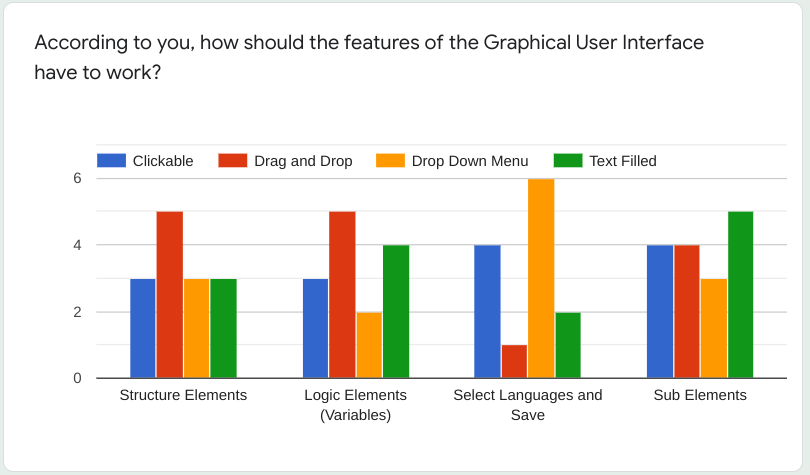
\includegraphics[width=0.55\linewidth]{../../Showcase-Work_Completed/Surveying/q11.png}
\captionof{figure}{\color{Green} Survey Question 11 - Found at: \href{https://github.com/ShinkuKira21/VisualPro-FinalProject/blob/main/Showcase-Work_Completed/Surveying/q11.png}{Original Image}}
\label{fig:q-11}
\end{center}\vspace{1cm}

The black plots are performance, whereas the blue plots are preference. The preference shows `Hard Usability' at zero percent, `Moderate Usability' at seventy-nine point thirty-three percent and `Easy Usability' at thirty-nine percent. The performance shows `Hard Usability' at zero percent, `Moderate Usability' at fourty-four point five percent and `Easy Usability' at fifty-seven point five.

\begin{center}\vspace{1cm}
    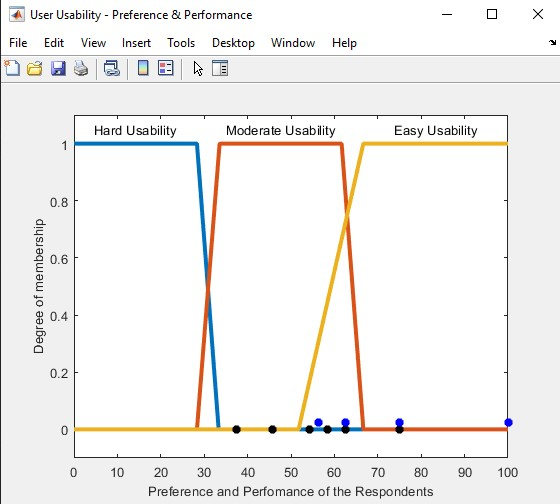
\includegraphics[width=0.45\linewidth]{FuzzyLogicPrefPerf.jpg}
    \captionof{figure}{\color{Green} Fuzzy Logic - Preference and Performance}
    \label{fig:fuzzyLogicPrefPerf}
\end{center}\vspace{1cm}

\begin{center}\vspace{1cm}
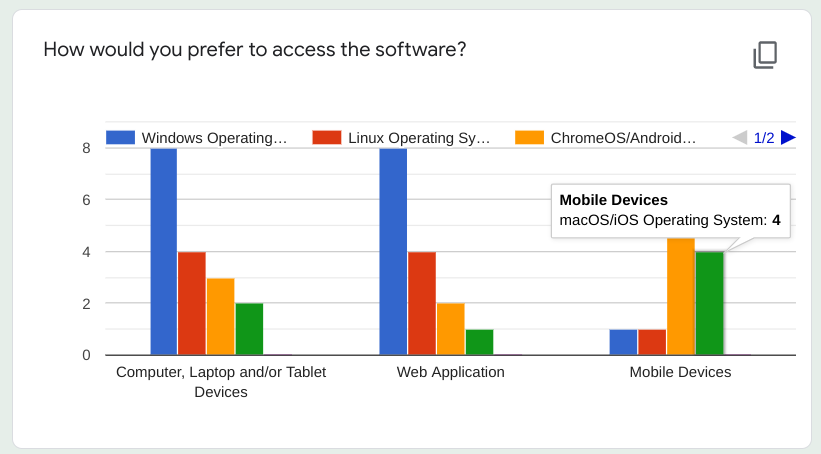
\includegraphics[width=0.55\linewidth]{../../Showcase-Work_Completed/Surveying/q12.png}
\captionof{figure}{\color{Green} Survey Question 12 - Found at: \href{https://github.com/ShinkuKira21/VisualPro-FinalProject/blob/main/Showcase-Work_Completed/Surveying/q11.png}{Original Image}}
\label{fig:q-12}
\end{center}\vspace{1cm}

%----------------------------------------------------------------------------------------
%	CONCLUSIONS
%----------------------------------------------------------------------------------------

\color{DarkRed} % SaddleBrown color for the conclusions to make them stand out

\section*{Conclusions}
By looking at the figure~\ref{fig:fuzzyLogicPrefPerf}, the performance suggests that the usability of VisualPro is `Moderate' usability, and the preference indicates that the usability is `Easy' usability. The preference suggests that the expectations were that the user usability should end up being easy-to-use, whereas the actual performance states that most users performed moderately well within the environment, where the rest of the users performed better. However, results do show a rough guide of the software's usability, which helps a project in a Iterative development methodology.

\color{DarkSlateGray} % Set the color back to DarkSlateGray for the rest of the content

%----------------------------------------------------------------------------------------
%	FORTHCOMING RESEARCH
%----------------------------------------------------------------------------------------

\section*{Forthcoming Research}

To further the understanding of the correlation between the two, perhaps trying this approach with the same or different research and development methodologies and converting the data into User Usability data. A comparison of the performance and preference could provide more information. However, this study shows an expectation of users' performance, which could impact the way projects are put together in the future. 
 %----------------------------------------------------------------------------------------
%	REFERENCES
%----------------------------------------------------------------------------------------

\nocite{*} % Print all references regardless of whether they were cited in the poster or not
\bibliographystyle{plain} % Plain referencing style
\bibliography{ref} % Use the example bibliography file sample.bib

%----------------------------------------------------------------------------------------
%	ACKNOWLEDGEMENTS
%----------------------------------------------------------------------------------------

\section*{Acknowledgements}
Appreciation goes out to the survey participants, which helped better understand how VisualPro may impact consumers in the future. Having the support from these participants helped advance the UI and UX progress of VisualPro.

%----------------------------------------------------------------------------------------

\end{multicols}
\end{document}